\documentclass[25pt, a0paper, portrait]{tikzposter}
\usepackage{tikz}
\usetikzlibrary{arrows.meta}
\usepackage{amsmath,amssymb,graphicx,xcolor,booktabs,colortbl}

% Colors
\definecolor{mainblue}{HTML}{1A3A5C}
\definecolor{accentblue}{HTML}{2E86AB}
\definecolor{softblue}{HTML}{D6EAF8}
\definecolor{softgreen}{HTML}{D5F5E3}
\definecolor{softyellow}{HTML}{FEF9E7}
\definecolor{softred}{HTML}{FADBD8}
\definecolor{softpurple}{HTML}{E8DAEF}

\usetheme{Default}
\colorlet{blocktitlebgcolor}{mainblue}
\colorlet{blocktitlefgcolor}{white}
\colorlet{blockbodybgcolor}{white}
\colorlet{titlebgcolor}{mainblue}
\colorlet{titlefgcolor}{white}

\newcommand{\cbox}[2]{\colorbox{#1}{\parbox{\dimexpr\linewidth-2\fboxsep}{\centering #2}}}

\title{\textbf{NeuroPathX}}
\author{DEGENEVE Hugo \qquad KAPOTOS Fotios}
\date{}
\institute{CentraleSupélec}

\begin{document}
\maketitle

% =========================================================
% MOTIVATION
% =========================================================
\block{Motivation}{
\large
\begin{itemize}
  \setlength\itemsep{0.4em}
  \item Autism spectrum disorder (ASD) and Alzheimer's disease (AD) arise from complex interactions between \textbf{genetics} and \textbf{brain structure} --- yet most methods treat them separately.
  \item Genetic variants (SNPs) can be aggregated into biologically meaningful \textbf{pathway scores}, linking molecular signals to known cellular functions.
  \item Structural MRI captures \textbf{macroscopic brain changes} associated with neurodegeneration and neurodevelopmental differences.
  \item \textbf{NeuroPathX} jointly models both modalities via a biologically-guided attention mechanism, enabling \textbf{interpretable classification} and discovery of pathway--brain region interactions.
\end{itemize}
}

% =========================================================
% PIPELINE
% =========================================================
\block{Pipeline}{
\begin{center}
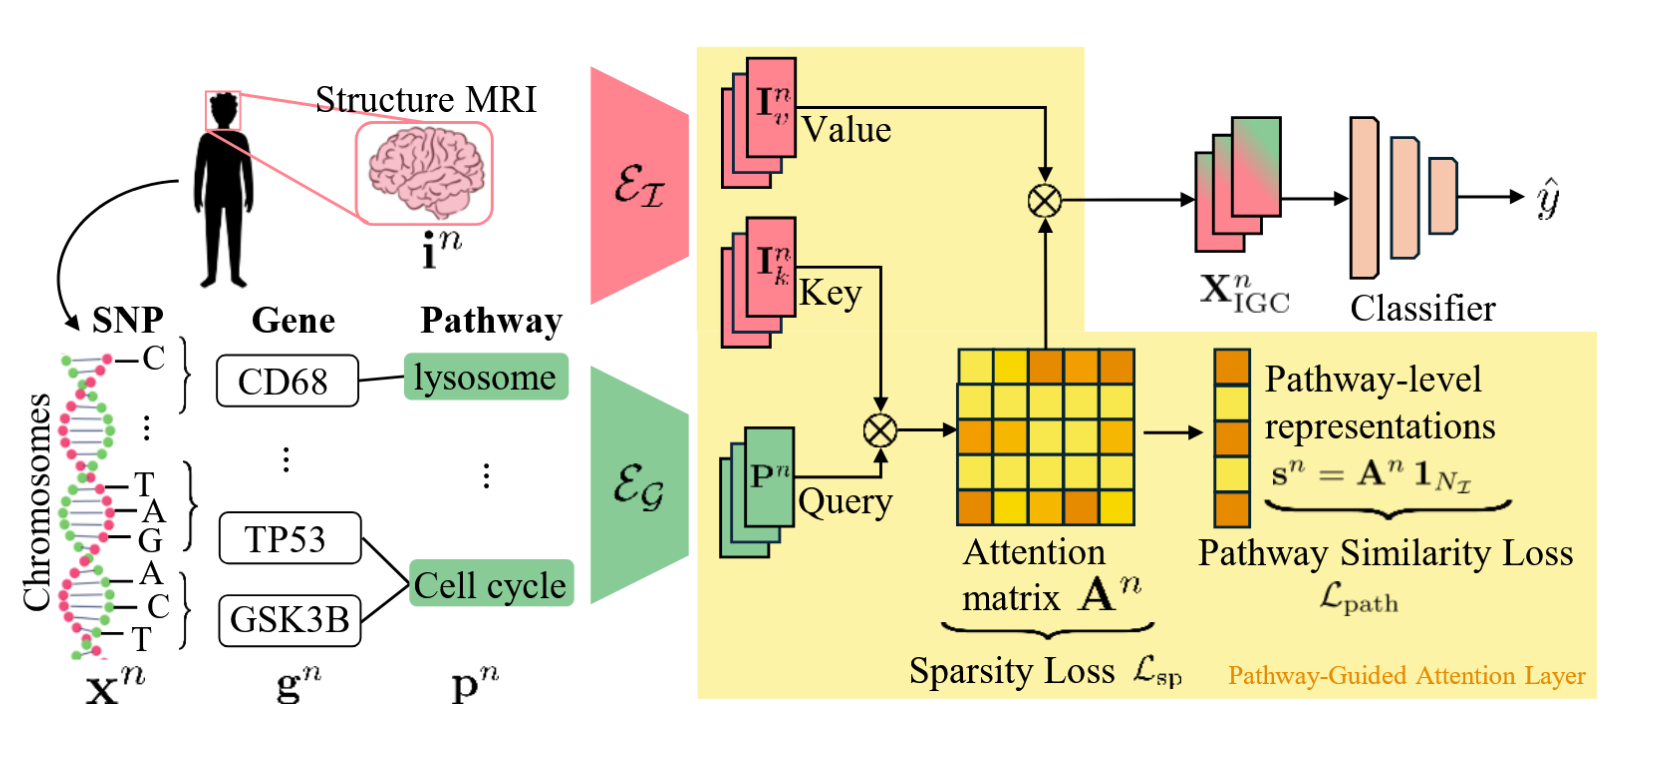
\includegraphics[width=0.6\linewidth]{dlmi.png}
\end{center}
}

% =========================================================
% TWO MODALITIES
% =========================================================
\begin{columns}

\column{0.5}
\block{Genetic Representation}{
\begin{center}
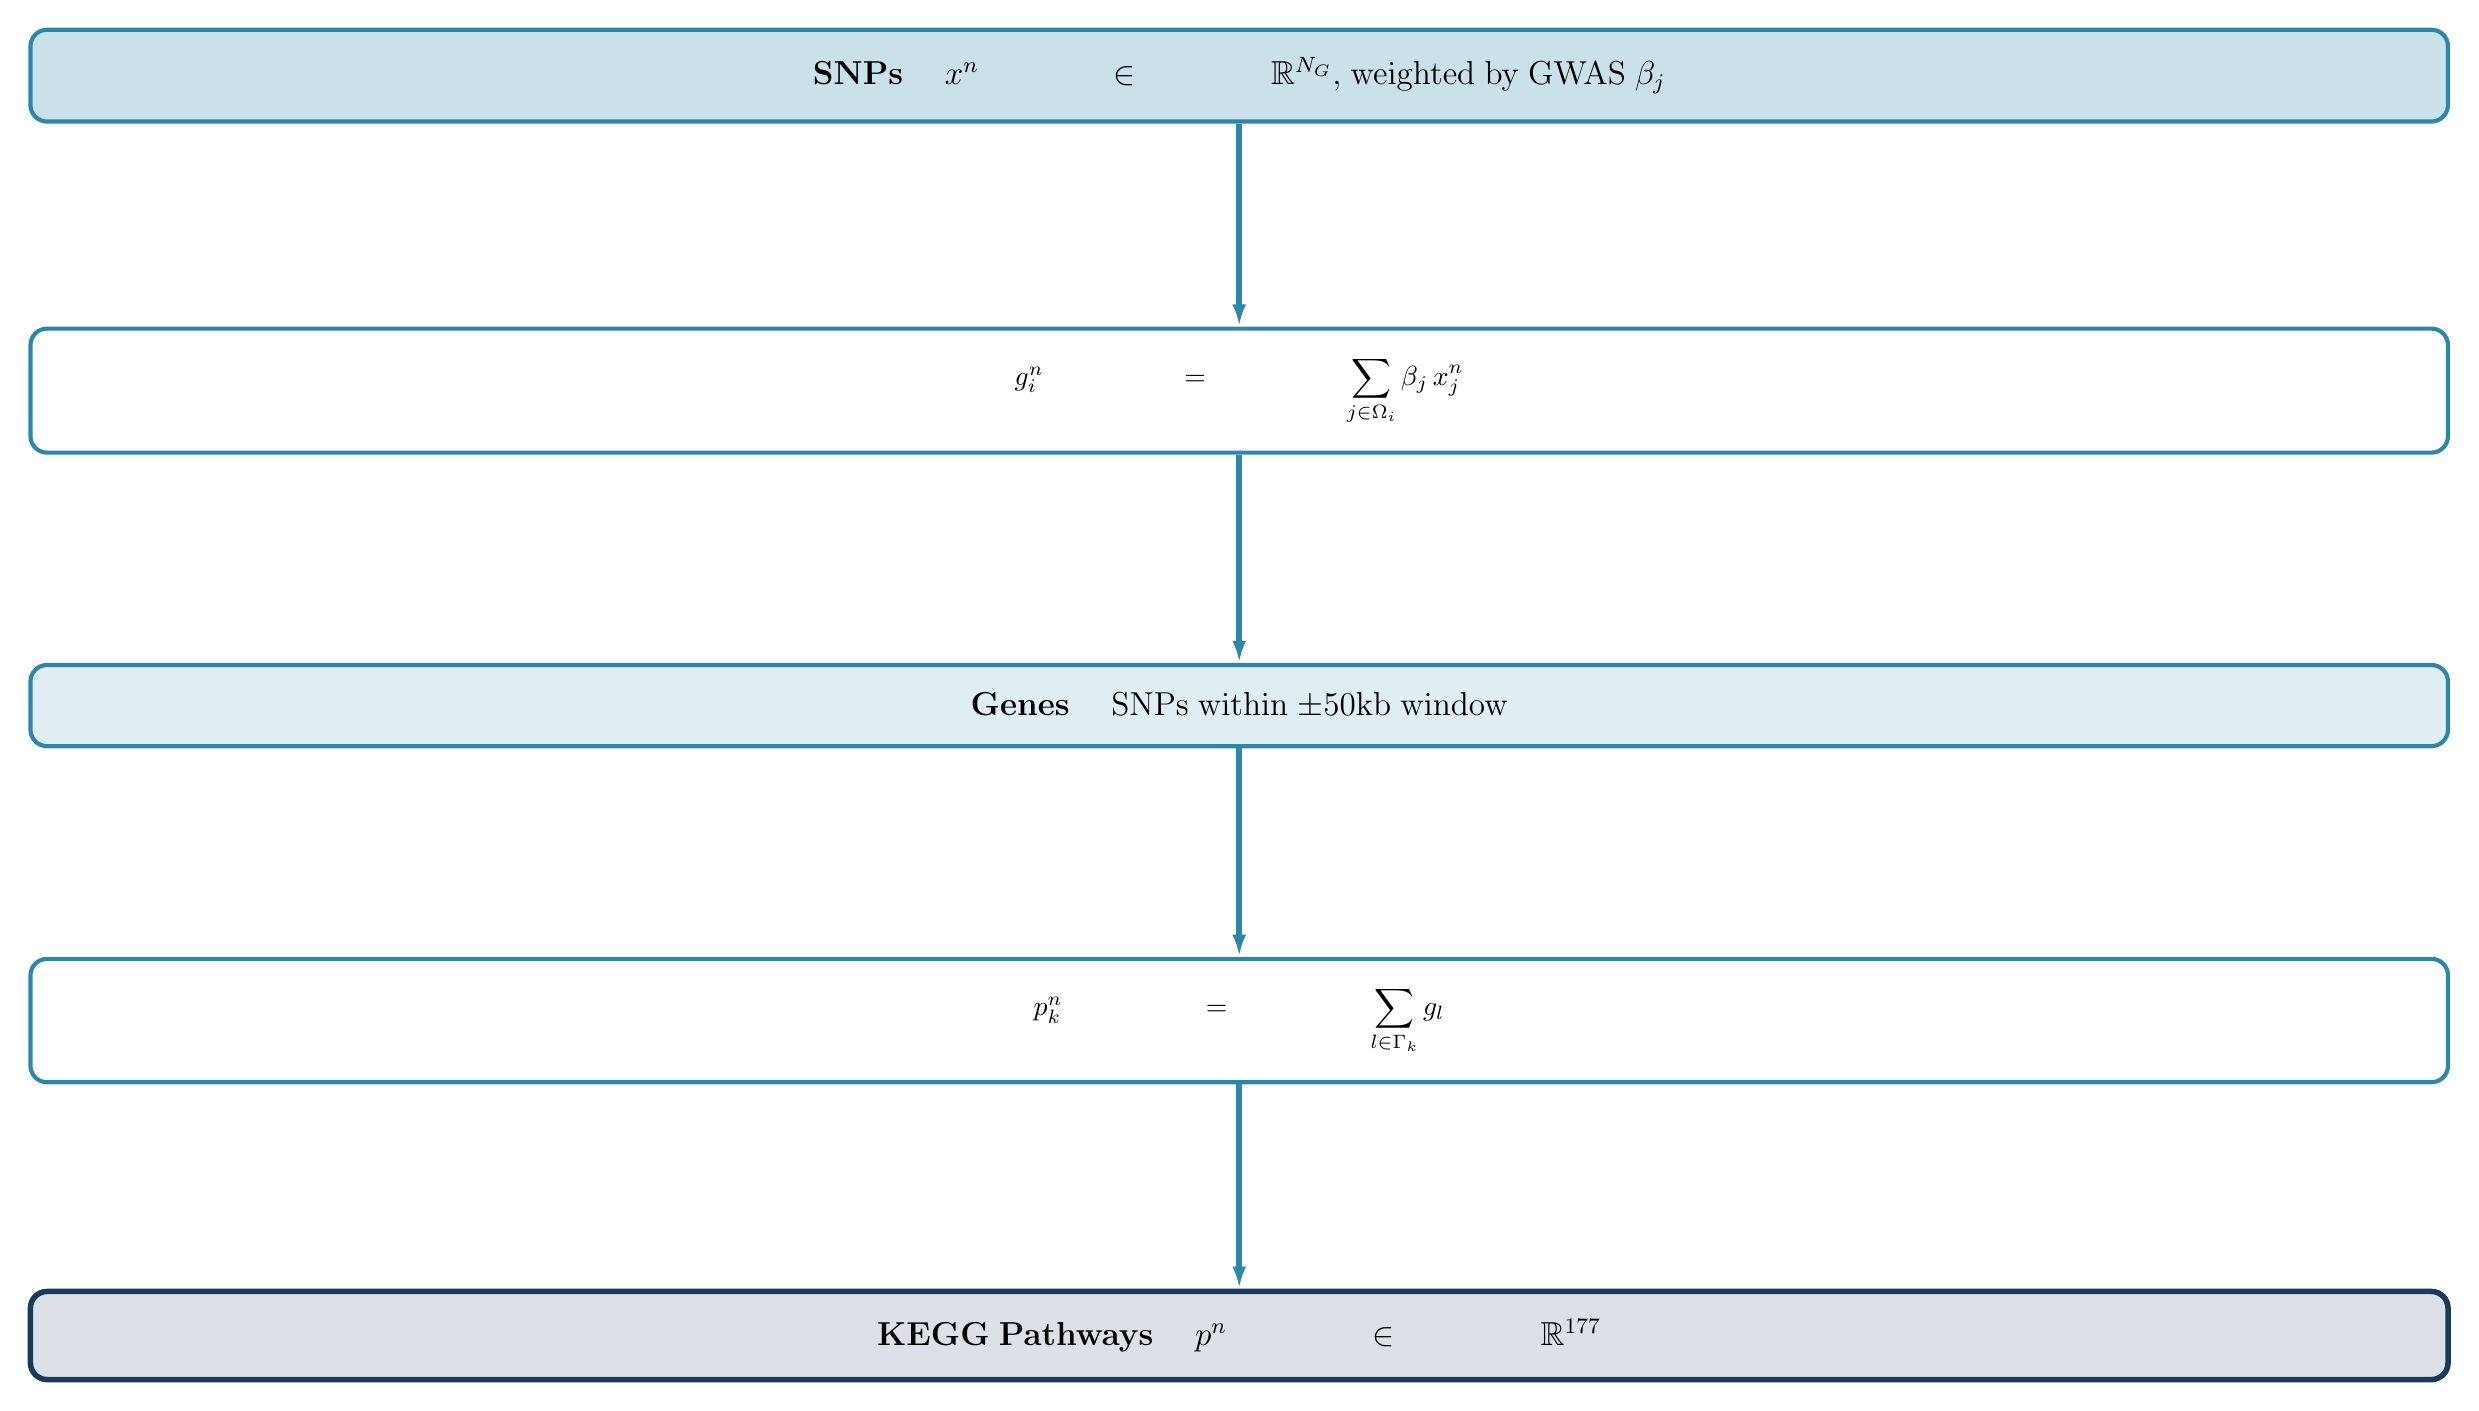
\begin{tikzpicture}[x=1cm, y=1cm,
  box/.style={draw=accentblue, rounded corners=6pt, line width=1.5pt, align=center, inner sep=10pt, text width=30cm},
  arr/.style={-{Latex[length=8pt,width=5pt]}, line width=2pt, accentblue}]

\node[box, fill=accentblue!25] at (15,0) (snp)
  {\large\textbf{SNPs} \quad $x^n \in \mathbb{R}^{N_G}$, weighted by GWAS $\beta_j$};

\node[box, fill=white] at (15,-4) (eq1)
  {$g^n_i = \displaystyle\sum_{j \in \Omega_i} \beta_j\, x^n_j$};

\node[box, fill=accentblue!15] at (15,-8) (gene)
  {\large\textbf{Genes} \quad SNPs within $\pm$50kb window};

\node[box, fill=white] at (15,-12) (eq2)
  {$p^n_k = \displaystyle\sum_{l \in \Gamma_k} g_l$};

\node[box, fill=mainblue!15, draw=mainblue, line width=2pt] at (15,-16) (out)
  {\large\textbf{KEGG Pathways} \quad $p^n \in \mathbb{R}^{177}$};

\draw[arr] (snp)--(eq1); \draw[arr] (eq1)--(gene);
\draw[arr] (gene)--(eq2); \draw[arr] (eq2)--(out);
\end{tikzpicture}
\end{center}
}

\column{0.5}
\block{MRI Representation}{
\begin{center}
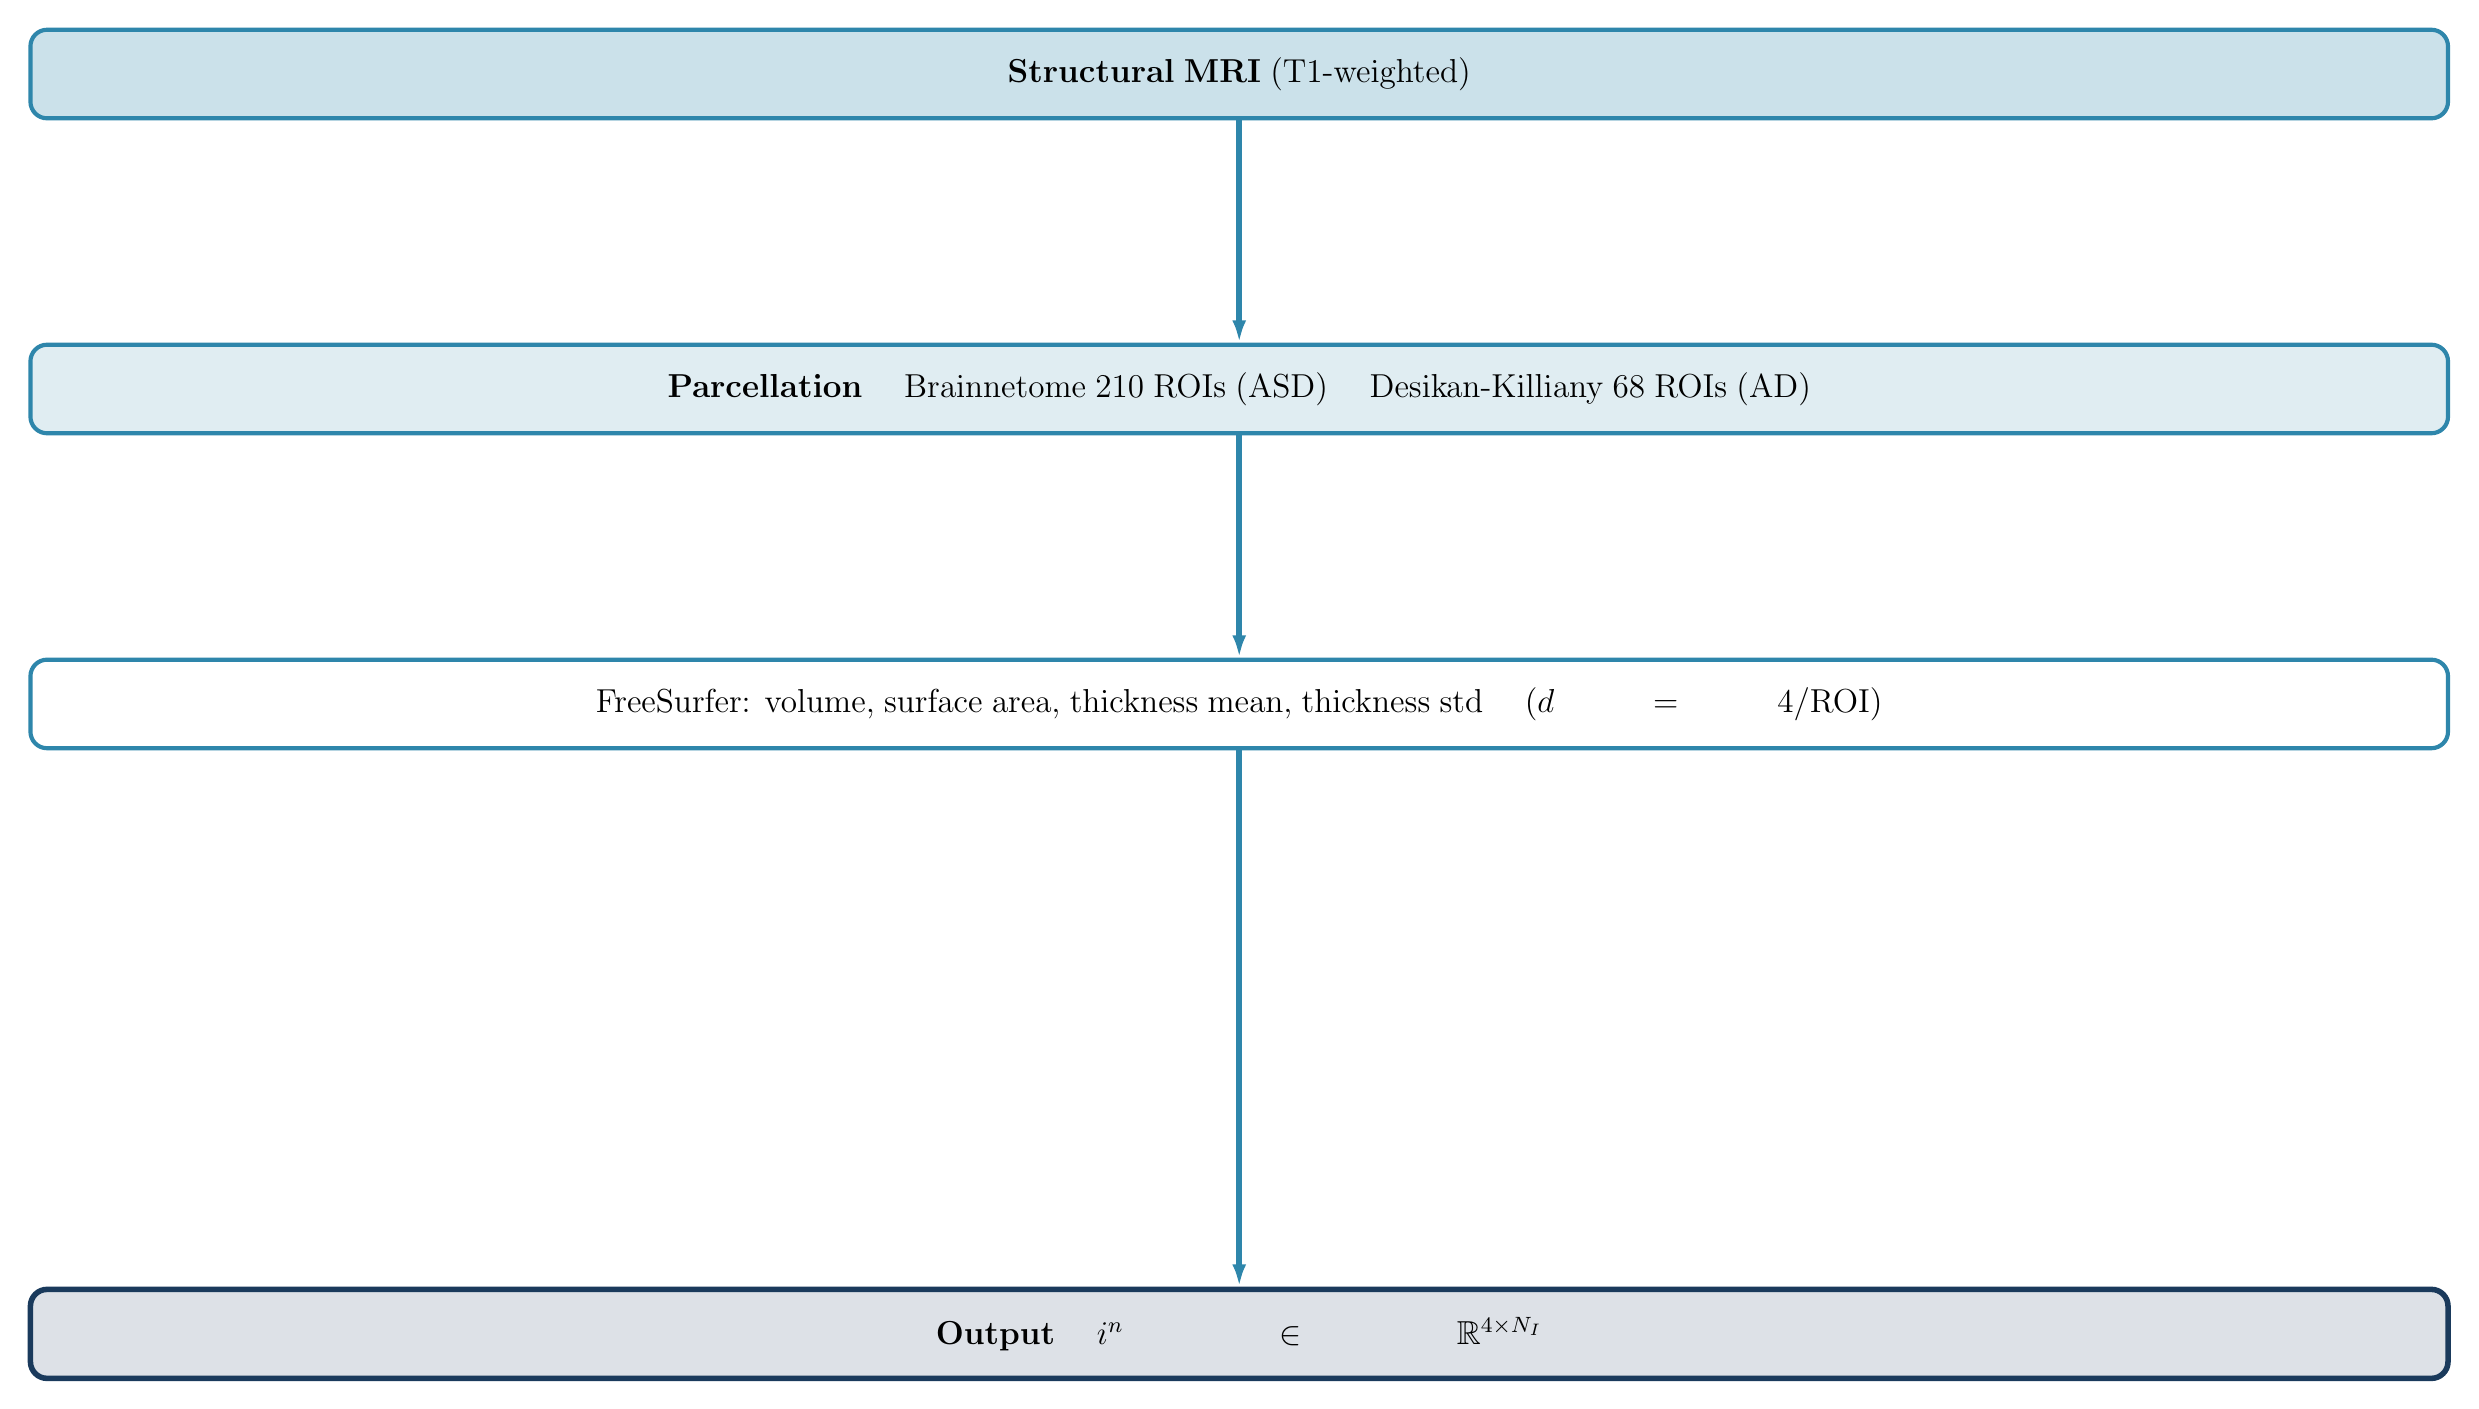
\begin{tikzpicture}[x=1cm, y=1cm,
  box/.style={draw=accentblue, rounded corners=6pt, line width=1.5pt, align=center, inner sep=10pt, text width=30cm},
  arr/.style={-{Latex[length=8pt,width=5pt]}, line width=2pt, accentblue}]

\node[box, fill=accentblue!25] at (15,0) (mri)
  {\large\textbf{Structural MRI} (T1-weighted)};

\node[box, fill=accentblue!15] at (15,-4) (atlas)
  {\large\textbf{Parcellation} \quad Brainnetome 210 ROIs (ASD) \quad Desikan-Killiany 68 ROIs (AD)};

\node[box, fill=white] at (15,-8) (feat)
  {\large FreeSurfer: volume, surface area, thickness mean, thickness std \quad ($d=4$/ROI)};

\node[draw=none, fill=none, text width=30cm, minimum height=2.2cm] at (15,-12) {};

\node[box, fill=mainblue!15, draw=mainblue, line width=2pt] at (15,-16) (out)
  {\large\textbf{Output} \quad $i^n \in \mathbb{R}^{4 \times N_I}$};

\draw[arr] (mri)--(atlas); \draw[arr] (atlas)--(feat); \draw[arr] (feat)--(out);
\end{tikzpicture}
\end{center}
}

\end{columns}
% =========================================================
% THREE LOSSES
% =========================================================
\begin{columns}

\column{0.333}
\block{Loss 1 --- Classification}{
\cbox{softblue}{\large\textbf{Weighted Cross-Entropy}}

\large Handles class imbalance between patients and controls.

\vspace{0.6em}
\[
\mathcal{L}_{\text{CE}} = \sum_n \Big[\delta\, y^n \log \hat{y}^n + (1{-}\delta)(1{-}y^n)\log(1{-}\hat{y}^n)\Big]
\]

\large $\delta$ controls class weighting; $y^n$ true label; $\hat{y}^n$ predicted.

\vspace{3.2em}
}

\column{0.333}
\block{Loss 2 --- Sparsity}{
\cbox{softgreen}{\large\textbf{Attention Sparsity (KL divergence)}}

\large Forces attention on the most salient pathway--brain interactions.

\vspace{0.6em}
\[
\mathcal{L}_{\text{sp}} = \sum_i \sum_j \mathrm{KL}\!\left(\mathrm{Ber}(q)\,\|\,\mathrm{Ber}(A^n_{ij})\right)
\]

\vspace{0.3em}
\large Target sparsity $q = 10^{-2}$. Applied to 2 random subjects per batch.
}

\column{0.333}
\block{Loss 3 --- Pathway Similarity}{
\cbox{softyellow}{\large\textbf{Cross-Cohort Consistency ($\ell_1$)}}
\large Encourages consistent pathway patterns across patients and controls.

\vspace{0.6em}
\[
\mathcal{L}_{\text{path}} = \frac{1}{M}\sum_{m=1}^{M} \left\| s^{(m)}_{\text{NC}} - s^{(m)}_{\text{PAT}} \right\|_1
\]

\vspace{0.3em}
\large $s^n = A^n \mathbf{1}_{N_I}$ (pathway influence); $M = 10$ pairs per epoch.
}

\end{columns}

% =========================================================
% RESULTS & LIMITATIONS
% =========================================================
\begin{columns}

\column{0.5}
\block{Results}{
\begin{center}
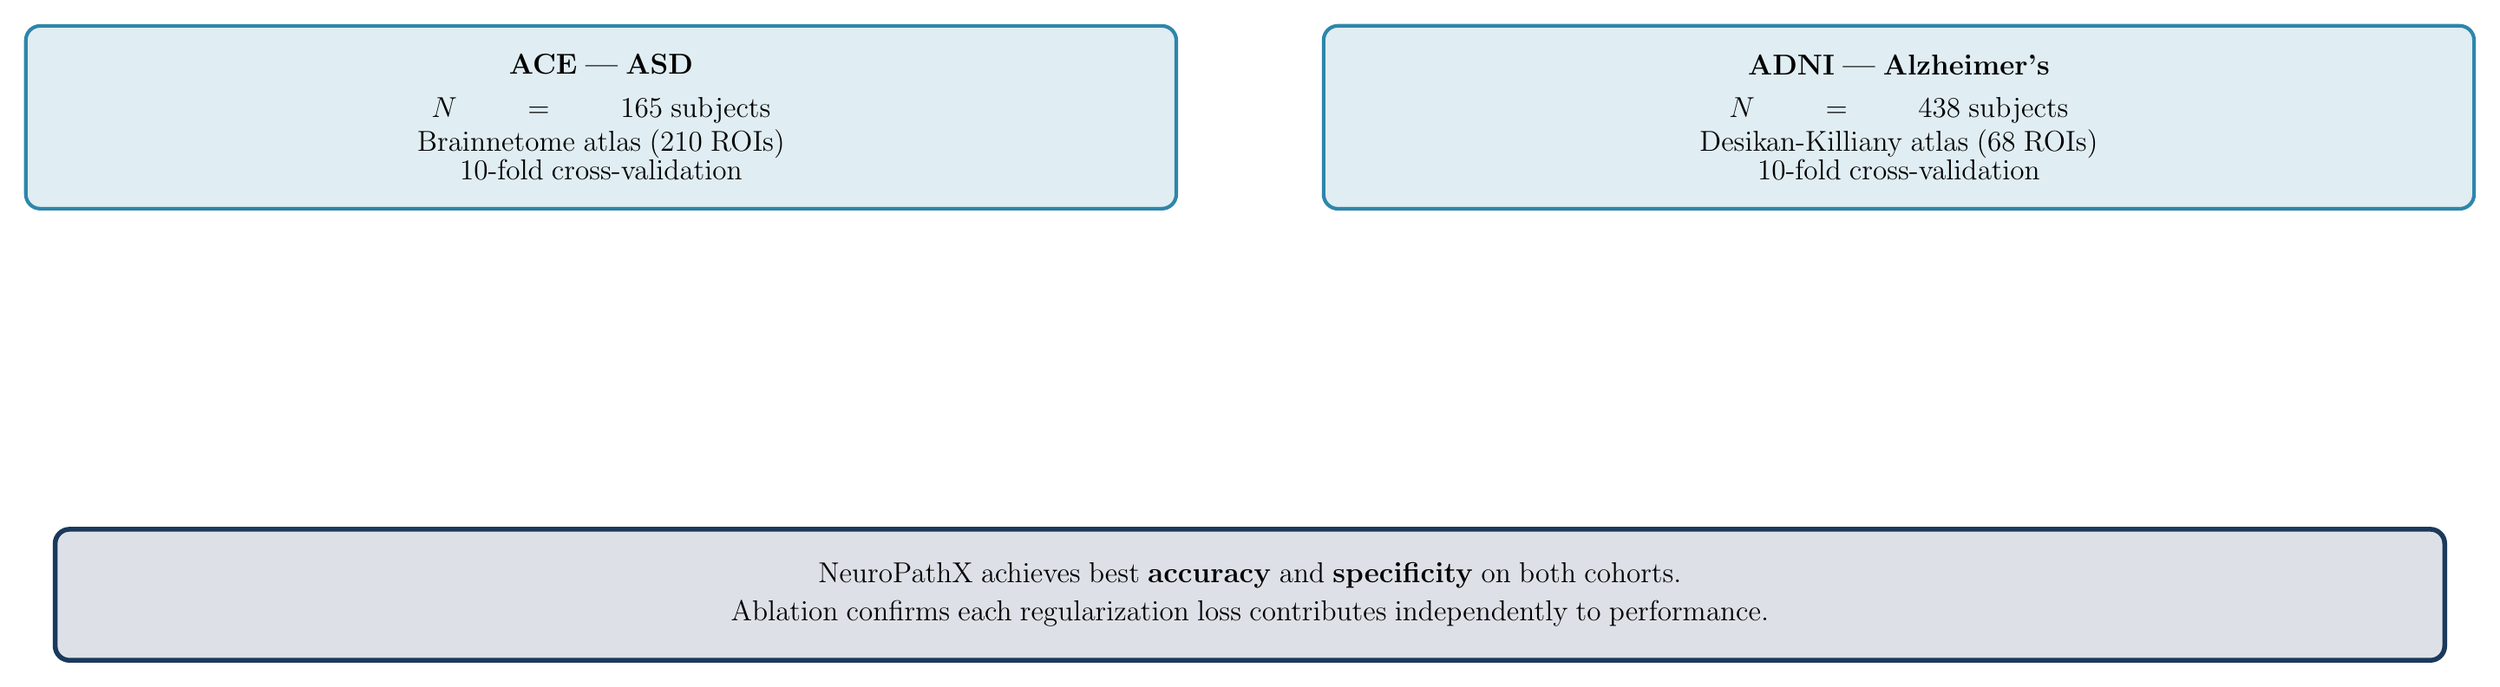
\begin{tikzpicture}[x=1cm, y=1cm,
  dbox/.style={draw=accentblue, rounded corners=6pt, line width=1.5pt, fill=accentblue!15, align=center, inner sep=12pt}]

\node[dbox, text width=16cm] at (9,0) (ace) {
  \large\textbf{ACE --- ASD}\\[4pt]
  $N = 165$ subjects\\
  Brainnetome atlas (210 ROIs)\\
  10-fold cross-validation
};
\node[dbox, text width=16cm] at (28,0) (adni) {
  \large\textbf{ADNI --- Alzheimer's}\\[4pt]
  $N = 438$ subjects\\
  Desikan-Killiany atlas (68 ROIs)\\
  10-fold cross-validation
};

\node[draw=mainblue, fill=mainblue!15, rounded corners=6pt, line width=2pt,
      text width=34cm, align=center, inner sep=14pt] at (18.5,-7) {
  \large NeuroPathX achieves best \textbf{accuracy} and \textbf{specificity} on both cohorts.\\[4pt]
  Ablation confirms each regularization loss contributes independently to performance.
};
\end{tikzpicture}
\end{center}
}

\column{0.5}
\block{Limitations \& Future Work}{
{\Large\textbf{Small datasets.}}\\
\large ACE ($N{=}165$) and ADNI ($N{=}438$) limit the stability of learned attention patterns.

\vspace{0.7em}
{\Large\textbf{Attention $\neq$ causation.}}\\
\large Weights reflect correlation, not causal biological relationships.

\vspace{0.7em}
{\Large\textbf{Fixed biological priors.}}\\
\large The $\pm$50kb window and KEGG pathways may miss context-dependent effects.

}

\end{columns}

\end{document}